\section{Résultats}

\begin{frame}
    \frametitle{Analyse de la Répartition des Sentiments}
    \begin{figure}
        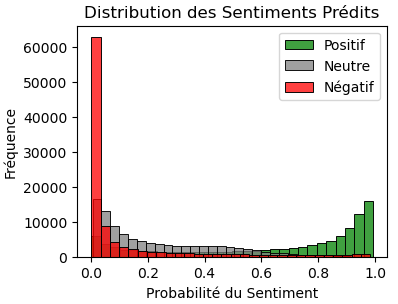
\includegraphics[scale=0.6]{Figures/distributionsentimentsRoberta.PNG}
        \caption{Distribution des Sentiments Prédits}
    \end{figure}
    L'histogramme des probabilités de sentiments prédites révèle des tendances distinctes dans la confiance du modèle.
\end{frame}

\begin{frame}
    \frametitle{Distribution des Sentiments Prédits par RoBERTa}
    \begin{figure}
        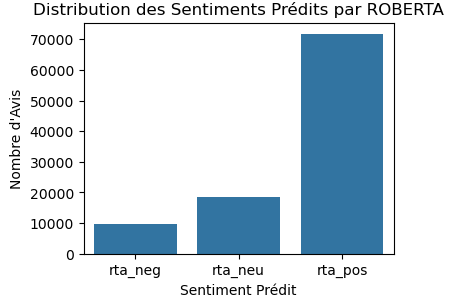
\includegraphics[scale=0.4]{Figures/distributiondessentimentRoberta.PNG}
        \caption{Distribution des Sentiments Prédits par RoBERTa}
    \end{figure}
    La répartition des sentiments prédits par RoBERTa sur l'ensemble de vos avis est la suivante :
    \begin{itemize}
        \item Sentiment Positif (rta\_pos) : 71,827 occurrences
        \item Sentiment Neutre (rta\_neu) : 18,492 occurrences
        \item Sentiment Négatif (rta\_neg) : 9,607 occurrences
    \end{itemize}
\end{frame}

\begin{frame}
    \frametitle{Distribution des Sentiments RoBERTa selon les Scores}
    \begin{figure}
        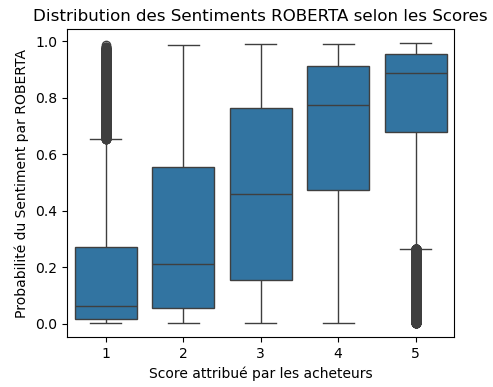
\includegraphics[scale=0.5]{Figures/sentimentrobertasurscore.PNG}
        \caption{Distribution des Sentiments RoBERTa selon les Scores}
    \end{figure}
    On constate que la distribution des prédictions de sentiment générées par le modèle RoBERTA, classées selon les scores attribués par les acheteurs.
\end{frame}

\begin{frame}
    \frametitle{Diagramme circulaire des proportions de sentiments}
    \begin{figure}
        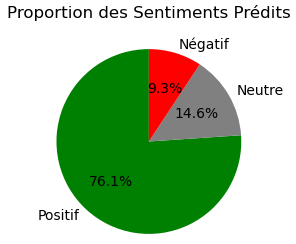
\includegraphics[scale=0.6]{Figures/proportiondessentimentspredits.PNG}
        \caption{Diagramme circulaire des proportions de sentiments}
    \end{figure}
    L'analyse des prédictions de sentiments révèle une tendance marquée vers des sentiments positifs, avec une majorité écrasante de 76.1% des prédictions appartenant à cette catégorie.
\end{frame}

\begin{frame}
    \frametitle{Analyse des Relations entre les Probabilités Prédites et les Scores Utilisateur}
    \begin{figure}
        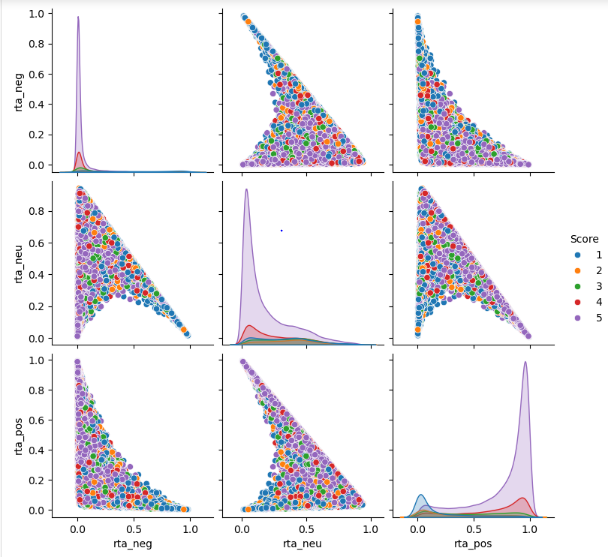
\includegraphics[scale=0.3]{Figures/robertaandscoreproba.PNG}
        \caption{Relation entre les Probabilités Prédites et les Scores Utilisateur}
    \end{figure}
    L'analyse des résultats met en évidence la distribution des probabilités prédites pour chaque sentiment (négatif, neutre, positif) en fonction des scores attribués par les utilisateurs.
\end{frame}

\begin{frame}
    \frametitle{Nuage de mots des avis positifs}
    \begin{figure}
        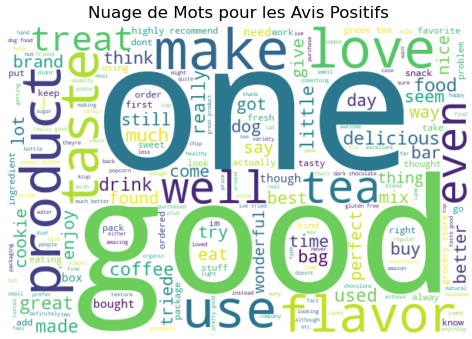
\includegraphics[scale=0.3]{Figures/wordcloudpositive.PNG}
        \caption{Nuage de Mots pour les Avis Positifs}
    \end{figure}
    Ce nuage de mots met en lumière les termes les plus fréquemment associés aux avis considérés comme positifs.
\end{frame}

\begin{frame}
    \frametitle{Nuage de mots des avis négatifs}
    \begin{figure}
        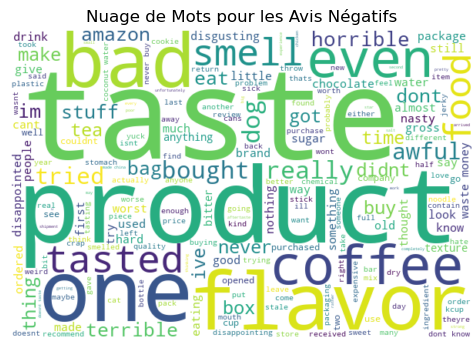
\includegraphics[scale=0.3]{Figures/wordcloudnegatif.PNG}
        \caption{Nuage de Mots pour les Avis Négatifs}
    \end{figure}
    De manière similaire, le nuage de mots représente les termes les plus fréquemment associés aux avis considérés comme négatifs par le modèle RoBERTa.
\end{frame}
